\documentclass[a4paper,10pt]{article}


%opening
\title{The Proof}
\author{}

\usepackage[active]{srcltx}

\usepackage{epsfig}
\usepackage{amsmath}
\usepackage{amsthm}
\usepackage{amssymb}
\usepackage{psfrag}
\usepackage[T1]{fontenc}
\usepackage{graphicx}
\usepackage{txfonts}

\newcommand{\w}{\omega}
\newcommand{\real}{Re}
\newcommand{\sgn}{\mathrm{sgn}}
\newcommand{\sinc}{\mathrm{sinc}}
\newcommand{\eps}{\epsilon}

\newtheorem{thm}{Theorem}[section]

\graphicspath{{../figure/}}


\begin{document}

\maketitle

\begin{thm}
Consider a proper SISO transfer function $G(s)=b(s)/a(s)$. Consider the set of all  nonlinearities lying in the gray area as represented in Figure~\ref{fig:sys}(b)
which can be mathematicall described in the following manner
\begin{align}
	\{n(t,\cdot)| 0\leq -n(t,y)\sgn(y)\leq N~~~\text{for all $t$,$y$ and}\\
		 n(t,y)y\leq -\alpha y^2 ~~~\text{for all $t$,$|y|<Y$} \} 
\end{align}

Assume that $G(s)$ is not positive real, that $a(s)-kb(s)$ has unstable roots for any sufficiently large $k>0$, and that $a(s)+kb(s)$ is stable for any $k\geq 0$.\\
Then it is not possible to show that the \textbf{positive} feedback interconnection of the two systems is absolutely stable using IQC/LMI techniques.
\end{thm}

~\\
~\\
\smallskip
Consider a non-positive real transfer function $G(s)$ with Nyquist plot (qualitatively) depicted in Figure~\ref{fig:sys}~(a) and the nonlinearity set in Figure~\ref{fig:sys}~(b).
\begin{figure}[hbt]
	\begin{tabular}{cc}
		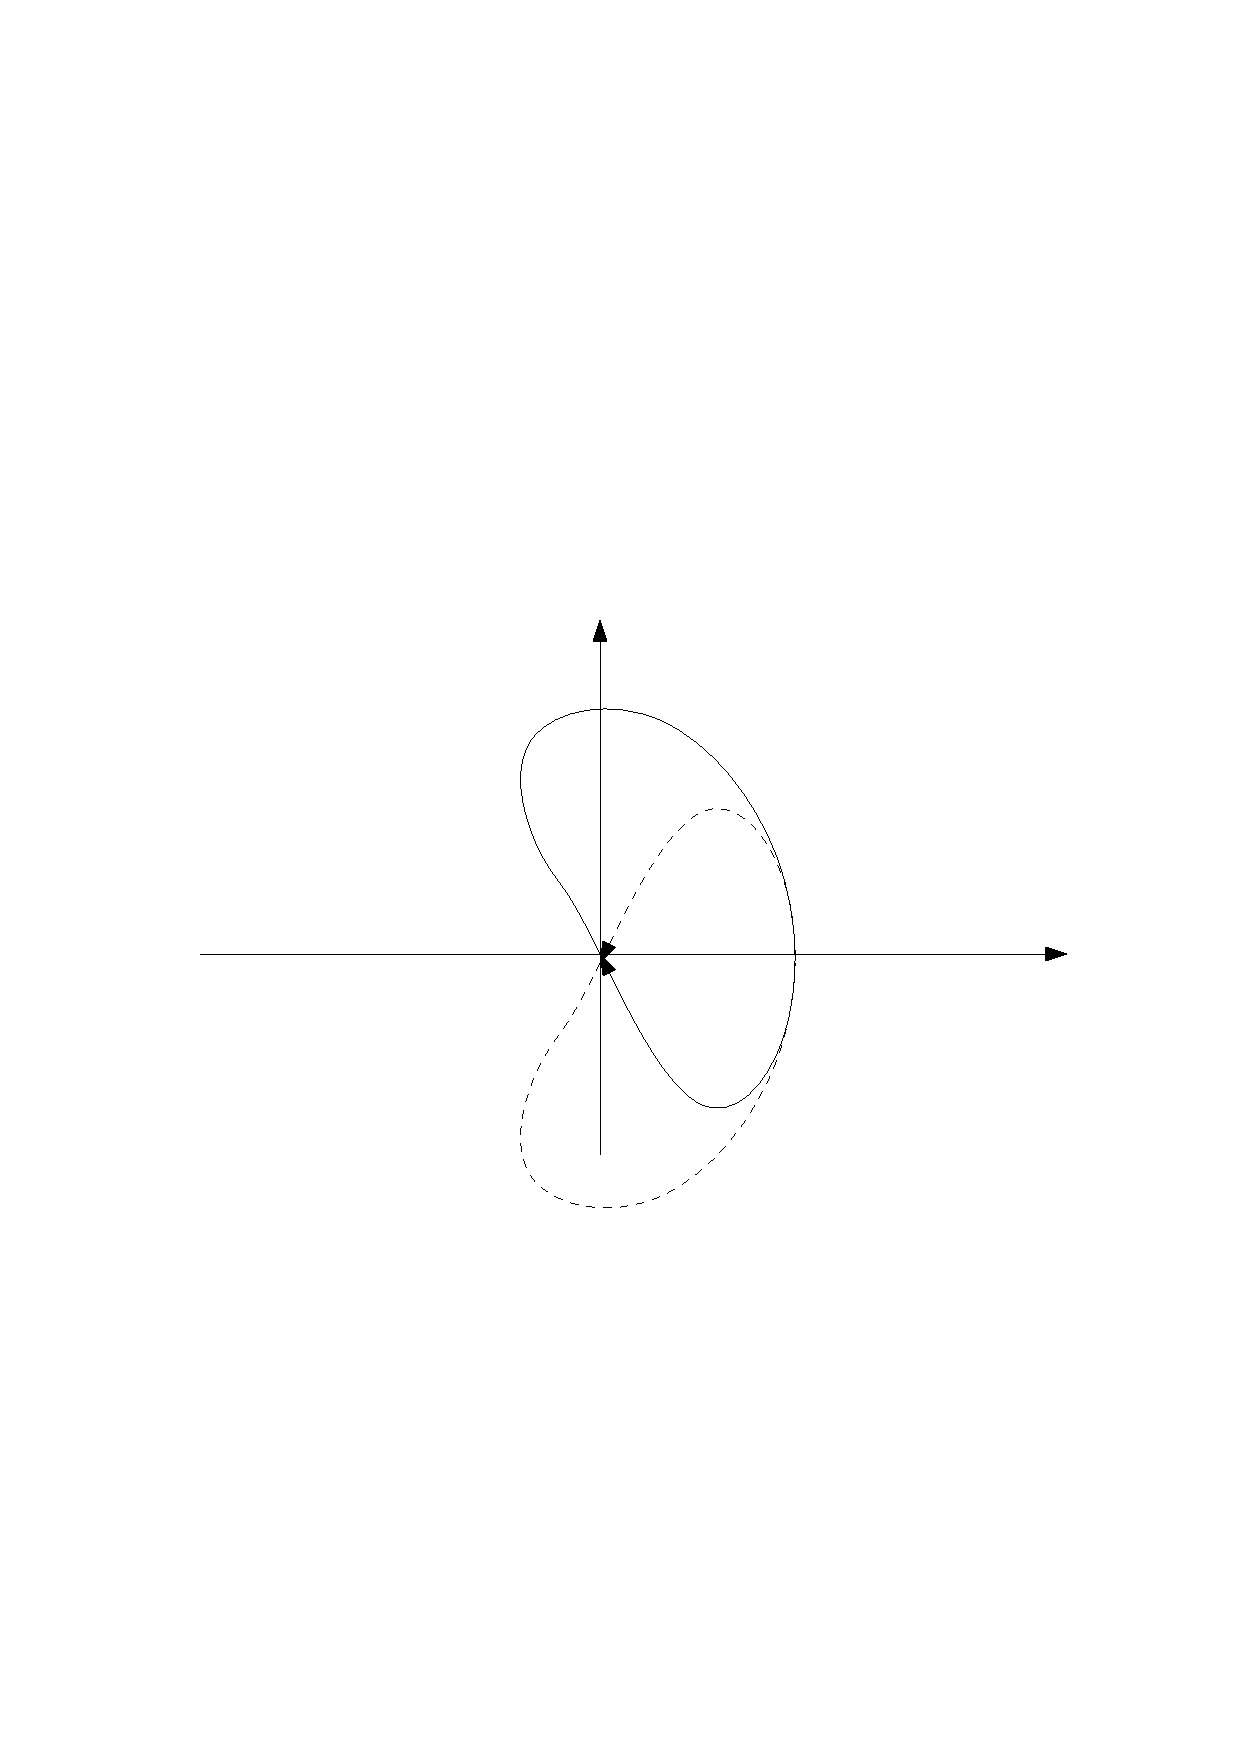
\includegraphics[width=0.45\columnwidth]{lin} 
	&
		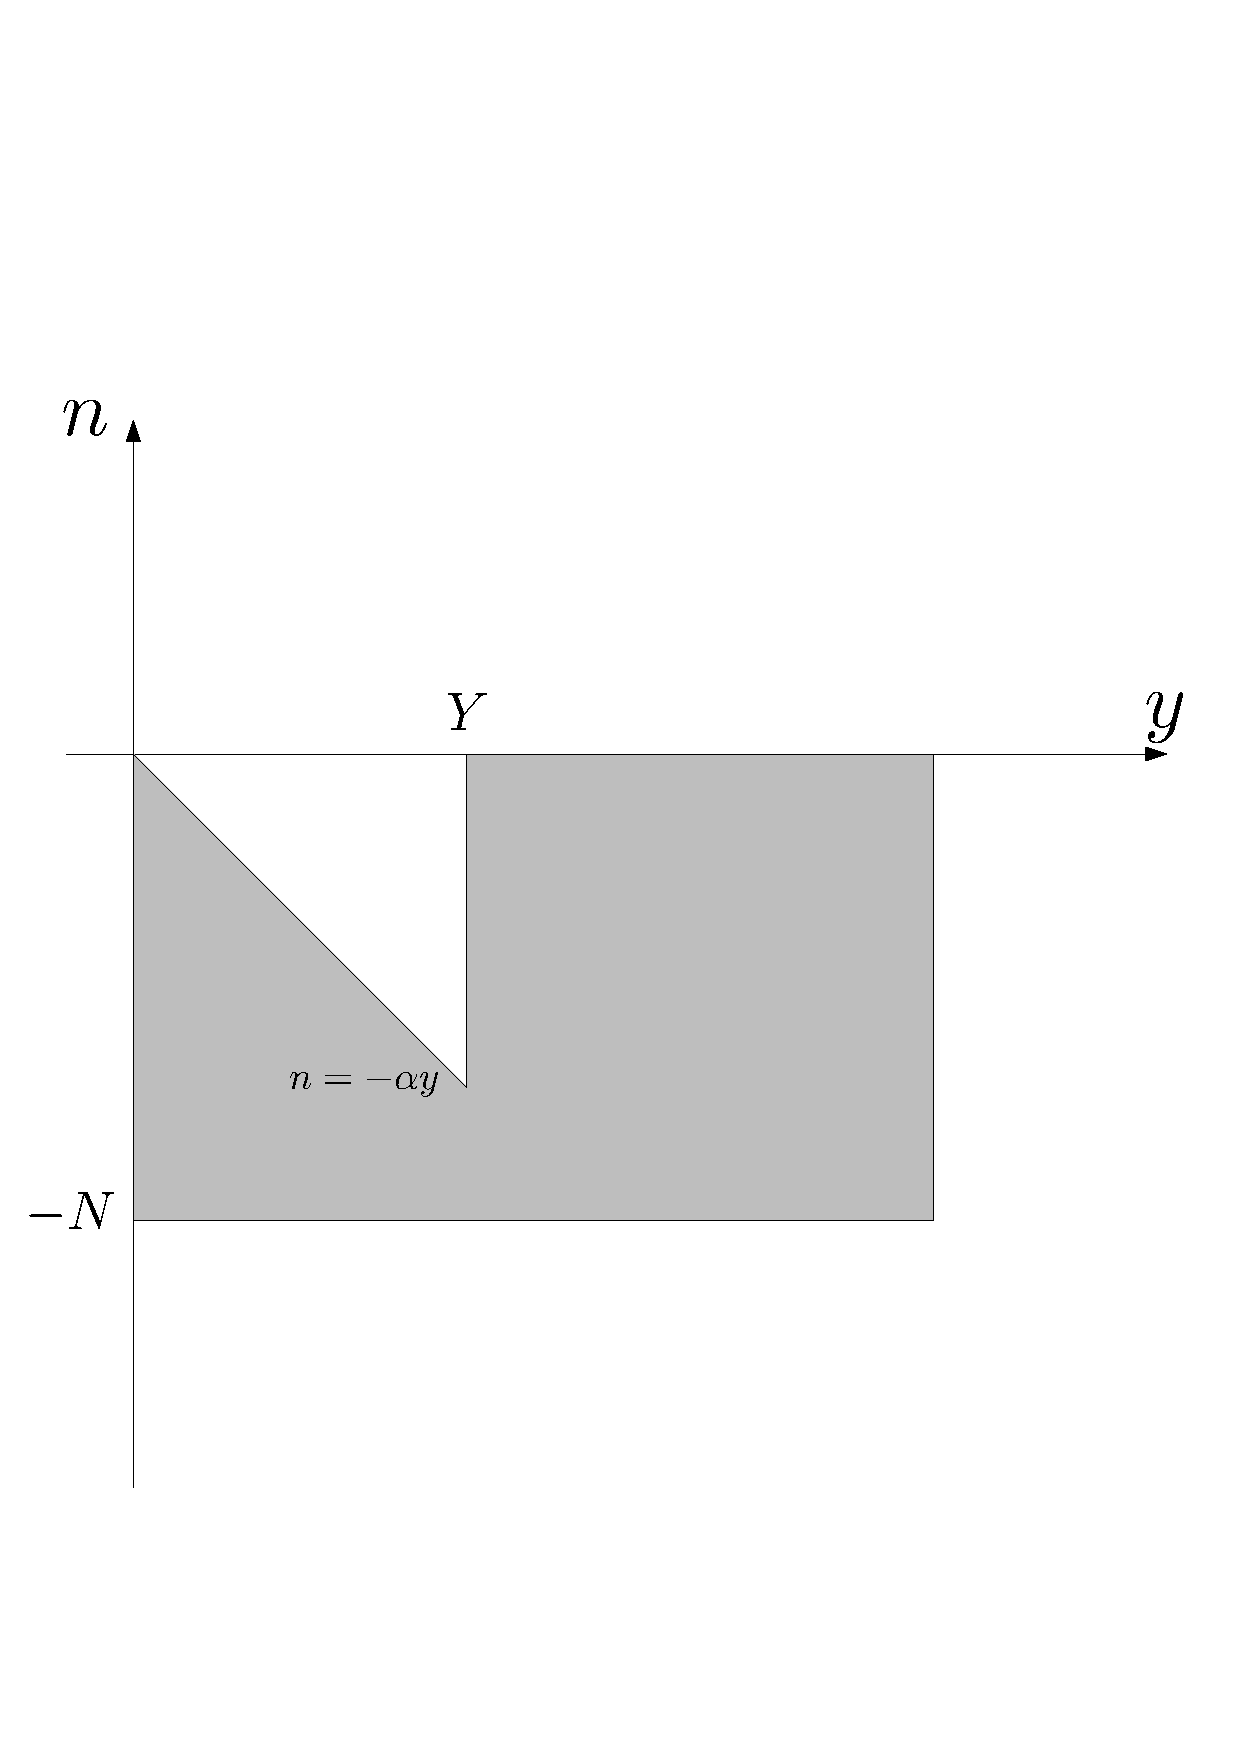
\includegraphics[width=0.45\columnwidth]{nonlin2}\\
	(a) & (b)
	\end{tabular}
	\caption{\label{fig:sys}}
\end{figure}


The statement will follow by contradiction.\\
Assume that it is possible to show the stability of the feedback interconnection using standard IQC/LMI techniques.
This means that there exists a Hermitian and bounded multiplier
\begin{align}
	\Pi(i\w)=
		\left(\begin{array}{cc}
			\Pi_{11}(i\w)	& \Pi_{12}(i\w)\\
			\Pi_{12}^*(i\w)	& \Pi_{22}(i\w)
		\end{array}\right)
\end{align}
where every $\Pi_{ij}(i\w)$ is a rational function of $i\w$ such that the following two conditions are satisfied
\begin{align}
	&\int_{\Re} \Pi_{11}(i\w) |\hat y(i\w)|^2+\Pi_{22}(i\w) |\hat \xi(i\w)|^2
		+ 2\real\{\Pi_{12}(i\w) \hat y(i\w)^*\hat \xi(i\w)  \}\geq 0
			& \forall y\in L_2 \label{eq:IQC} \\
	& \Pi_{11}(i\w) |G(i\w)|+\Pi_{22}(i\w) +2\real\{G^* \Pi_{12}(i\w)\}\leq -\eps
			& \forall \w, \exists \eps>0. \label{eq:KYP}
\end{align}
We will refer to the condition (\ref{eq:IQC}) as IQC-condition and to the condition (\ref{eq:KYP}) as KYP-condition.\\

Since $\Pi(i\w)$ is Hermitian  then we have that
\begin{align}
	Im\{\Pi_{11}(i\w)\}=Im\{\Pi_{22}(i\w)\}=0
		&\qquad \text{for any } \w
\end{align}
Since the two diagonal entries also need to be rational bounded functions of $i\w$, they must be constant
\begin{align}
	\Pi_{11}(i\w)\}=\Pi_{11}; &\qquad \Pi_{22}(i\w)=\Pi_{22}.
\end{align}


\section{A key lemma}
Define
\begin{align}
% 	\gamma_m(\w_0,t):=\sqrt{\frac{\w_0}{\pi}}\cos(\w_0 t) \chi_{[0, mT]}(t)
	\gamma_m(\w_0,t):=\cos(\w_0 t) \chi_{[0, 2m\pi/\w_0]}(t)
% 	\gamma(\w_0,t):=\cos(\w_0 t) \chi_{[0, 2\pi/\w_0]}(t)
\end{align}
for any $\w_0\neq 0$ and $m$ positive integer, where $\chi_{A}(\cdot)$ is the characteristic function of a set $A$.
Consider a $2\pi/\w_0-$periodic complex signal $s(t)$, espress it in its Fourier series, that is
\begin{align}
	s(t)=\sum_{j=-\infty}^{+\infty}S_k e^{ik\w_0 t}.
\end{align}
where $S_l$ are the Fourier coefficients and define
\begin{align}
	s_m=s(t)\chi_{[0, 2m\pi/\w_0]}(t)
\end{align}
\begin{thm}
	It holds that
	\begin{align}
		\lim_{m\rightarrow +\infty}
			\frac{\w_0}{m\pi}\int \hat \gamma_m(\w)^* \Phi(i\w) \hat s_m(\w)d\w=
				\frac{1}{2}\left(\Phi(-i\w_0)S_{-1}+\Phi(i\w_0)S_1\right)
	\end{align}
\end{thm}
\begin{proof}
	\begin{align}
		\hat s_m(\w) &= \sum_{l}S_l\delta(\w-l\w_0)*
			\frac{m\pi}{\w_0}\sinc\left(m\pi\frac{\w}{\w_0}\right)\\
		&= \frac{m\pi}{\w_0}
			\sum_{l}S_l \sinc\left(m\pi\frac{\w-l\w_0}{\w_0}\right)
	\end{align}

	\begin{align}
		\hat \gamma_m= \frac{m\pi}{\w_0}
			\left[
				\frac{1}{2}\sinc\left(m\pi\frac{\w-\w_0}{\w_0}\right)+
				\frac{1}{2}\sinc\left(m\pi\frac{\w+\w_0}{\w_0}\right)
			\right]
	\end{align}
	Then
	\begin{align*}
% 		\lim_{m\rightarrow +\infty}
		&\frac{\w_0}{m\pi}\int \hat \gamma_m(\w)^* \Phi(i\w) \hat s_m(\w)d\w=\\
		&\quad = \frac{m\pi}{\w_0} \int \Phi(i\w)
			\left[
				\frac{1}{2}\sinc\left(m\pi\frac{\w-\w_0}{\w_0}\right)+
				\frac{1}{2}\sinc\left(m\pi\frac{\w+\w_0}{\w_0}\right)
			\right]
			\sum_{l}S_l \sinc\left(m\pi\frac{\w-l\w_0}{\w_0}\right)d\w=\\
		&\quad=\int \Phi\left(\frac{\w_0\alpha}{m\pi}\right)
			\left[
				\frac{1}{2}\sinc\left(\alpha-m\pi\right)+
				\frac{1}{2}\sinc\left(\alpha+m\pi\right)
			\right]
			\sum_{l}S_l \sinc\left(\alpha-lm\pi\right)d\alpha=\\
		&\quad= \frac{1}{2}\int\Phi\left(\frac{\w_0\alpha}{m\pi}+\w_0\right)
				\sinc(\alpha)
				\sum_{l}S_l \sinc\left(\alpha-(l-1)m\pi\right)d\alpha+\\
		&\qquad +\frac{1}{2}\int\Phi\left(\frac{\w_0\alpha}{m\pi}-\w_0\right)
				\sinc(\alpha)
				\sum_{l}S_l \sinc\left(\alpha-(l+1)m\pi\right)d\alpha
	\end{align*}
	When $m$ goes to $+\infty$ the integral of the product of two $\sinc(\cdot)$ functions goes to zero for any $l\neq 1$ in the first integral and for any $l\neq -1$ in the second.
	Then
	\begin{align*}
		&\lim_{m\rightarrow +\infty}
		\frac{\w_0}{m\pi}\int \hat \gamma_m(\w)^* \Phi(i\w) \hat s_m(\w)d\w=\\
		&\quad= \frac{1}{2}\Phi(\w_0)S_{1}\int\sinc(\alpha)^2d\alpha+
			\frac{1}{2}\Phi(-\w_0)S_{-1}\int\sinc(\alpha)^2 d\alpha
	\end{align*}
\end{proof}



\section{Conditions on $\Pi_{ij}$}

\subsection{$\Pi_{22} \leq 0$}
By contradiction $\Pi_{22}=q>0$.\\
Consider the operator
\begin{align}
	n=ky
\end{align}
for $k>0$.
For any $y\in L_2$, the IQC-condition is
\begin{align}
	\|y\|^2\int_{\Re} \Pi_{11} + 2k\real\{\Pi_{12}(i\w)\} +qk^2  \geq 0.
\end{align}
Since $\Pi_{12}(i\w)$ is a bounded matrix, we have that, for $k$ sufficiently large, the IQC is satisfied. This, along with the KYP-condition, implies that the connection is stable. Then we have a contradiction because, by hypothesis, for $k$ sufficiently large the interconnection is also unstable.\\


\subsection{$\Pi_{22} = 0$}
By contradiction $\Pi_{22}=-q<0$.\\
Consider the operator
\begin{align}
	n=-\sgn(y)\max\{N,ky\}.
\end{align}
which must satisfy the IQC-condition for any $k>\alpha$ and for any $y\in L_2$.
Choosing 
\begin{align}
	y(t)=\frac{N}{k}\chi_{[0,1]}(t),
\end{align} 
the IQC-condition is
\begin{align}
	0 &\leq \Pi_{11}\frac{N^2}{k^2}-qN^2+2\int_{\Re}
		\real\{\hat y(\w)^*\Pi_{12 }(i\w)\hat n(\w)\}\leq \\
	& \leq \Pi_{11}\frac{N^2}{k^2}-qN^2 +\|\Pi_{12}(i\w)\|_{\infty}\frac{N^2}{k}
\end{align}
For $k$ sufficiently large we obtain a contradiction, then $\Pi_{22}=0$. \\

\subsection{$\real\{\Pi_{12}(i\w)\leq 0$ for any $\w$}
Consider the operator
\begin{align}
	n=-\sgn(y)\max\{N,ky\}.
\end{align}
which must satisfy the IQC-condition for any $k>\alpha$ and for any $y\in L_2$.
Choosing 
\begin{align}
	y(t)=\frac{N}{k}\gamma_m(\w_0,t),
\end{align} 
the IQC-condition is
\begin{align}
	0 &\leq \frac{m\pi}{\w_0}\frac{N^2}{k^2}\Pi_{11}+
		2\real\int_{\Re}\{\hat y(\w)^*\Pi_{12 }(i\w)\hat n(\w)\}= \\
	& = \frac{m\pi}{\w_0}\frac{N^2}{k^2}\Pi_{11}-
		2\frac{m\pi}{\w_0}\frac{N^2}{k}\real\left\{\int_{\Re}\hat \gamma_m(\w_0,\w)^*\Pi_{12 }(i\w)\hat \gamma_m(\w_0,\w)\right\} =\\
\end{align}
Assume by contradiction that $\real\{\Pi_{12}(i\w_0)\}>q>0$. In such a case, by the key lemma, it is possible
to find $m$ large enough such that
\begin{align}
	0 \leq \frac{m\pi}{\w_0}\frac{N^2}{k^2}\Pi_{11}-
		2\frac{m\pi}{\w_0}\frac{N^2}{k}q.
\end{align}
% 
% 	& = \frac{\pi}{\w_0}\frac{N^2}{k^2}\Pi_{11}-\frac{\pi}{\w_0}\frac{N^2}{k}\real\{\Pi_{12}(\w_0)\}
Then, choosing $k$ large enough we obtain a contradiction.

\subsection{$\Pi_{11} \geq 0$}
By contradiction $\Pi_{11}=-q<0$\\
Consider the operator
\begin{align}
	n=-\sgn(y)\max\{N,\alpha y\}
\end{align}
which must satisfy the IQC-condition and choose
\begin{align}
	y(t)=A\chi_{[0,1]}(t).
\end{align}
with $A>N/\alpha$.
The IQC-condition is
\begin{align}
	-qA^2 +2AN\int_{\Re}\real\{\sinc^2(\w)\Pi_{12}(i\w)\}  \geq 0.
\end{align}
which is not satisfied for A large enough (because the integral is bounded). This is a contradiction, then $\Pi_{11}\geq 0$.

\subsection{$Im\{\Pi_{12}(\w)\} = 0$ for any $\w$}
By contradiction assume that
\begin{align}
	\Pi_{12}(\w_0)=|\Pi_{12}(\w_0)|e^{i\phi_0}
\end{align}
with $\phi_0 \neq -(2l+1)\pi$. Since $\real\{\Pi_{12}(\w_0)\}\leq 0$, we can assume, without loss of generality, $\phi_0 \in [\pi/2,3\pi/2]$ with $\phi_0\neq \pi$.
Consider the input signal
\begin{align}
	y(t)=A\gamma_m(\w_0,t)
\end{align}
with $A<Y$ and the two operators
\begin{align}
	n_a(y)=
		\left\{\begin{array}{ll}
			-N	& \qquad \text{if } 0<y<\eps A \text{ and } \dot y>0\\
			N	& \qquad \text{if } -\eps A<y<0 \text{ and } \dot y<0\\
			\alpha A\sgn(y) & \qquad \text{otherwise}
		\end{array}\right.
\end{align}
\begin{align}
	n_b(y)=
		\left\{\begin{array}{ll}
			-N	& \qquad \text{if } 0<y<\eps A \text{ and } \dot y<0\\
			N	& \qquad \text{if } -\eps A<y<0 \text{ and } \dot y>0\\
			\alpha A\sgn(y) & \qquad \text{otherwise}
		\end{array}\right.
\end{align}
The wave forms of $n_a(y(t))$ and $n_b(y(t))$ do not depend on $A$ and are represented in figure.
\begin{figure}
	\centering
	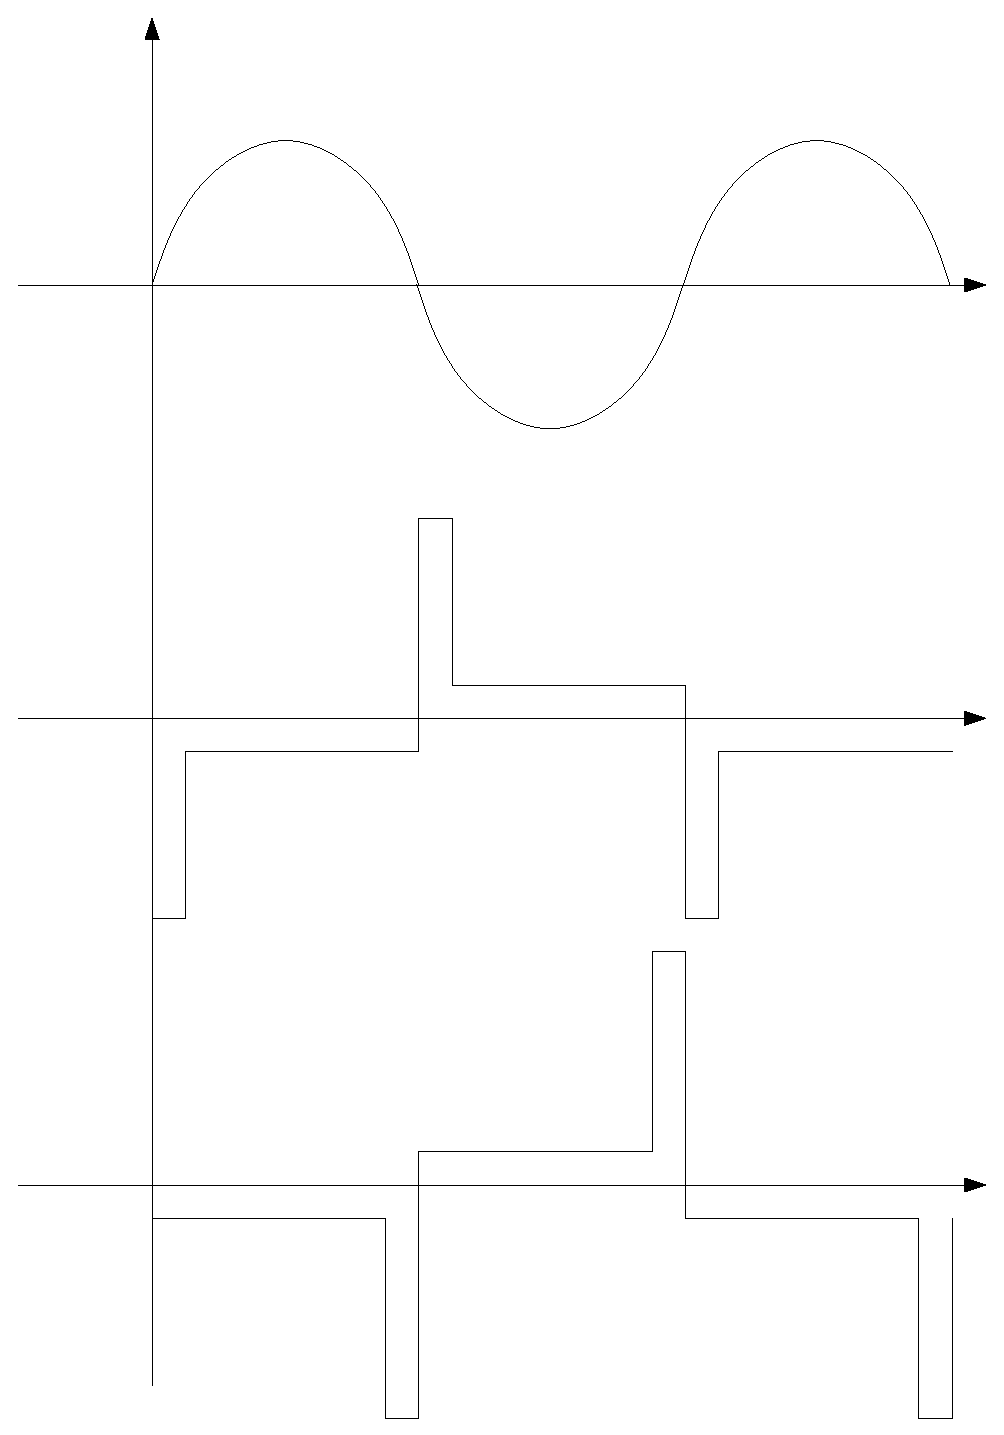
\includegraphics[width=0.7\columnwidth]{PhaseDestroying}
\end{figure}
Choose 
\begin{align}
	0<\eps=\arcsin(\psi)
\end{align}
and evaluate the Fourier coefficients $S_1^{a}, S_1^{b}$ of the two square waves $n_a(A\cos(\w t))$ and $n_a(A\cos(\w t))$.
\begin{align}
	S_1^{a}=2(N-\alpha A)(\cos(\psi)-1+i\sin(\psi))+4\alpha A \\
	S_1^{b}=2(N-\alpha A)(\cos(\psi)-1-i\sin(\psi))+4\alpha A
\end{align}
Note that, for any $\eta>0$, it is possible to choose $A$ and $\psi$ small enough such that 
\begin{align}
 	\pi/2 < \arg(S_1^{a}) < \pi/2+\eta\\
	3\pi/2-\eta < \arg(S_1^{b}) < 3\pi/2
\end{align}
The IQC-condition for $n_a$ becomes (for $m$ large)
\begin{align}
	0&\leq A^2\frac{m\pi}{\w_0}\Pi_{11} +
		2A\real\left\{\int_{\Re}\hat\gamma_m(\w_0,\w)\Pi_{12}(i\w)\hat n_{a}(\w)
			\right\}=\\
	&= A^2\frac{m\pi}{\w_0}\Pi_{11} +
		2A\frac{m\pi}{\w_0}\real\{\Pi_{12}(i\w_0)S_1^a+ \Pi_{12}(-i\w_0)S_{-1}^a\}=\\
	&= A^2\frac{m\pi}{\w_0}\Pi_{11} + 
		2A\frac{m\pi}{\w_0}\real\{|\Pi_{12}(i\w_0)||S_1^a|e^{i(\phi_0+\arg(S_1^a))}\}
\end{align}
Considering a small $A$, the quadratic term becomes negligible compared to the linear one, yielding 
\begin{align}
	\cos(\phi_0+\arg(S_1^a))\geq 0\Rightarrow \cos(\phi_0+\pi/2)\geq 0.
\end{align}
Repeating the same argument with $n_b$ we find that
\begin{align}
	\cos(\phi_0+\arg(S_1^B))\geq 0 \Rightarrow \cos(\phi_0+3\pi/2)\geq 0
\end{align}
which is a contradiction. This proves the assertion.

\section{Final step}
Summarizing, the multiplier $\Pi(i\w)$ must be of the form
\begin{align}
	\Pi(i\w)=
		\left(\begin{array}{cc}
			\Pi_{11}	& \Pi_{12}(i\w)\\
			\Pi_{12}(i\w)	& 0
		\end{array}\right)
\end{align}
with $\Pi_{11}\geq 0$ and $\Pi_{12}(i\w)\leq 0$.
The KYP condition is
\begin{align}
\Pi_{11}(i\w) |G(i\w)|^2 +2\real\{G^* \Pi_{12}(i\w)\}\leq -\eps
			& \qquad \forall \w
\end{align}
that implies
\begin{align}
	\Pi_{12}(i\w) 2\real\{G \} \leq -\eps & \qquad \forall \w
\end{align}
and this can not be verified because it requires $G(i\w)$ positive real.

\end{document}
